\documentclass[class=minimal,border=0pt]{standalone}

\usepackage{tikz}
\usepackage{fontspec}

\setmainfont[
  Scale=0.90,
  BoldFeatures={Scale=1.0}
]{Open Sans}

\def\cols{
    {},
    {},
    {},
    {2},
    {5},
    {1,2,1},
    {2,1,2},
    {16},
    {2,1,2},
    {1,3,1},
    {5},
    {3},
    {},
    {},
    {},
    {}
}

% (sublists have to be REVERSED so the for loop makes sense!!!)
\def\rows{
    {1},
    {3},
    {5},
    {1},
    {3,1},
    {3,1,1},
    {3,1,3},
    {1,1,3},
    {1,1,1},
    {1,1,1},
    {2,1},
    {2},
    {1},
    {3},
    {3},
    {1}
}

\begin{document}

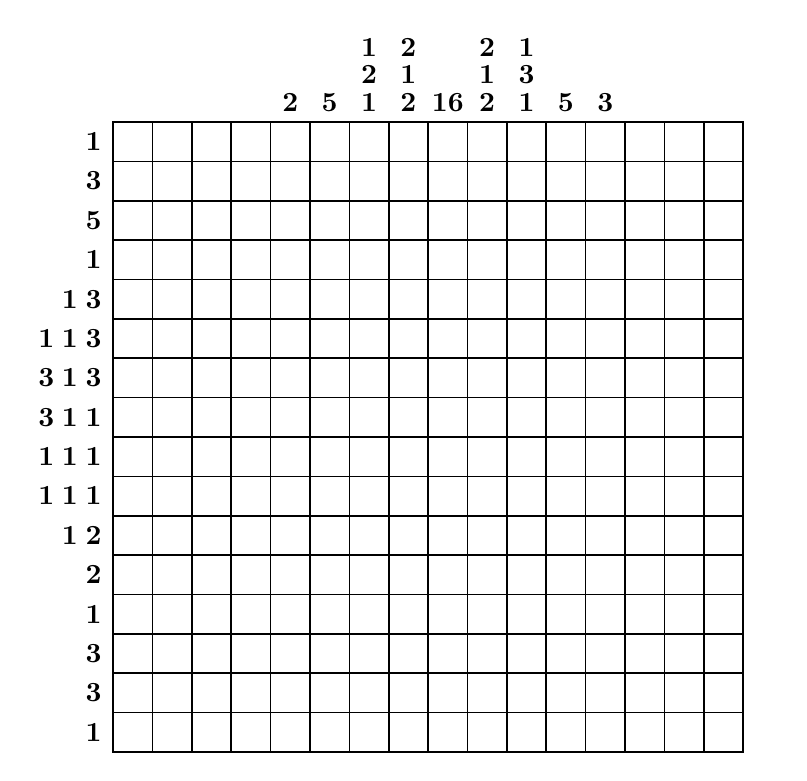
\begin{tikzpicture}[
    every node/.style={rectangle, draw=black, semithick, minimum size=5mm, node font=\bfseries},
    num/.style={draw=none, minimum size=4mm}
]
  \node
    foreach \list [count=\x] in \cols
      foreach \val [count=\y] in \list
        [num] at (\x/2, 0.35*\y+0.15) {\val};
  \node
    foreach \list [count=\y] in \rows
      foreach \val [count=\x] in \list
        [num] at (-0.3*\x-0.2, 0.5-\y/2) {\val};

  % grid
  \node
    foreach \a [count=\y] in \rows
      foreach \b [count=\x] in \cols
        at (\x/2-0.5, 0.5-\y/2) {};

\end{tikzpicture}

\end{document}
